\chapter{Enumeration Mapping}
\label{cha:enumerations}

	While the mapping of common data types is mostly clear we have to 
	take a special look to enumerations. Enumeration is a type where 
	numeric constants are represented by alphanumeric keywords or even 
	descriptions. For developers the enum data type is a way to make 
	the source code more readable. But most databases do not provide 
	this type.

	%-----
	\section{Enum data type}
		The enum data type has values given at compile time. If you want 
		to change the values it is needed to recompile the code. Independent 
		from how the mapping to the database is done there will ever be 
		the problem of assuring the database consistency.
		
		An object state 
		like shown in Listing \ref{lst:enumObjectState} is a place where 
		enumeration makes really sense, because it makes the code much 
		more readable.
		
		\begin{lstlisting}[float=hbt,language={[Sharp]C},caption=Object state with enumeration,label=lst:enumObjectState]
public class DomainObject
{
	public enum ObjectState {Unchanged, Modified, Added, Deleted, Detached}

	private ObjectState m_state = ObjectState.Detached;

	internal ObjectState State     
	{
		get { return m_state; }
		set { m_state = value; }
	}
}
		\end{lstlisting}
		
		If you don't want to run into problem you should use enumerators only 
		for internal purposes never mapped to the database.	Also the user of a 
		program should never see any values of an enum.


	\section{Current mapping}
	
		The existing HsrOrderApp uses the enum type for a person role. In Figure
		\ref{fig:AnalysisEnumOld}	you can see the PersonRole table mapping PersonIDs 
		to a RoleName. The value of the enum is written to the database as a string
		for each assignment. 
		
		\begin{figure}[hbt]
			\begin{center}
				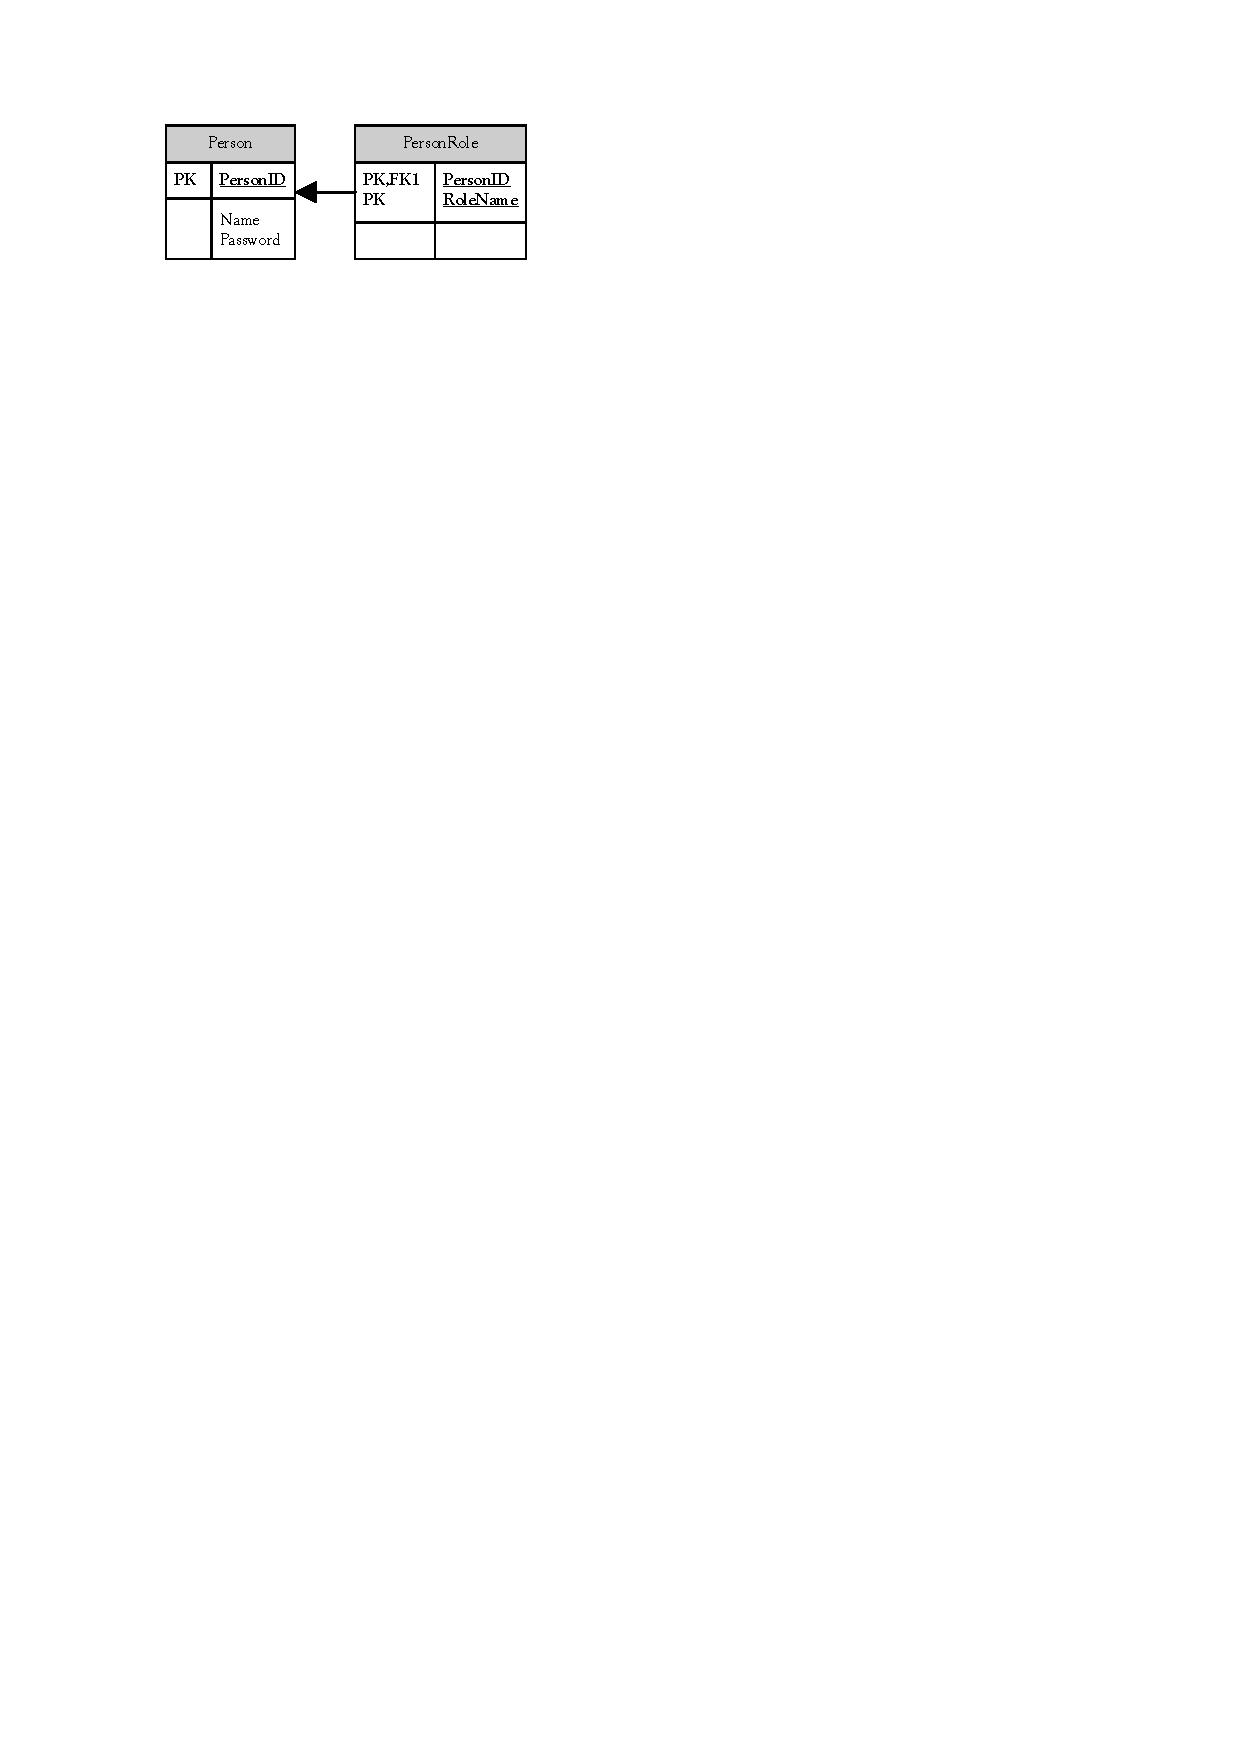
\includegraphics{./files/inc/figures/AnalysisEnumOld}
				\caption{\label{fig:AnalysisEnumOld} existing database}
			\end{center}
		\end{figure}
		
		This is a bad database design because the strings are saved redundant. But not
		only that. You will also run into big troubles if you want to add, change or delete
		values of the enumerator. Every change must be done in the code and on the database 
		to assure the consistency between enum values and database entries.
		
	%-----
	\section{Normalized design}
	
		In a fully normalized database each string should be only saved once 
		referenced by a unique id like you can see in Figure \ref{fig:AnalysisEnumNew}. 
		There every role description exists exactly once. The table PersonRole now 
		only maps RoleIDs to PersonIDs.

		\begin{figure}[hbt]
			\begin{center}
				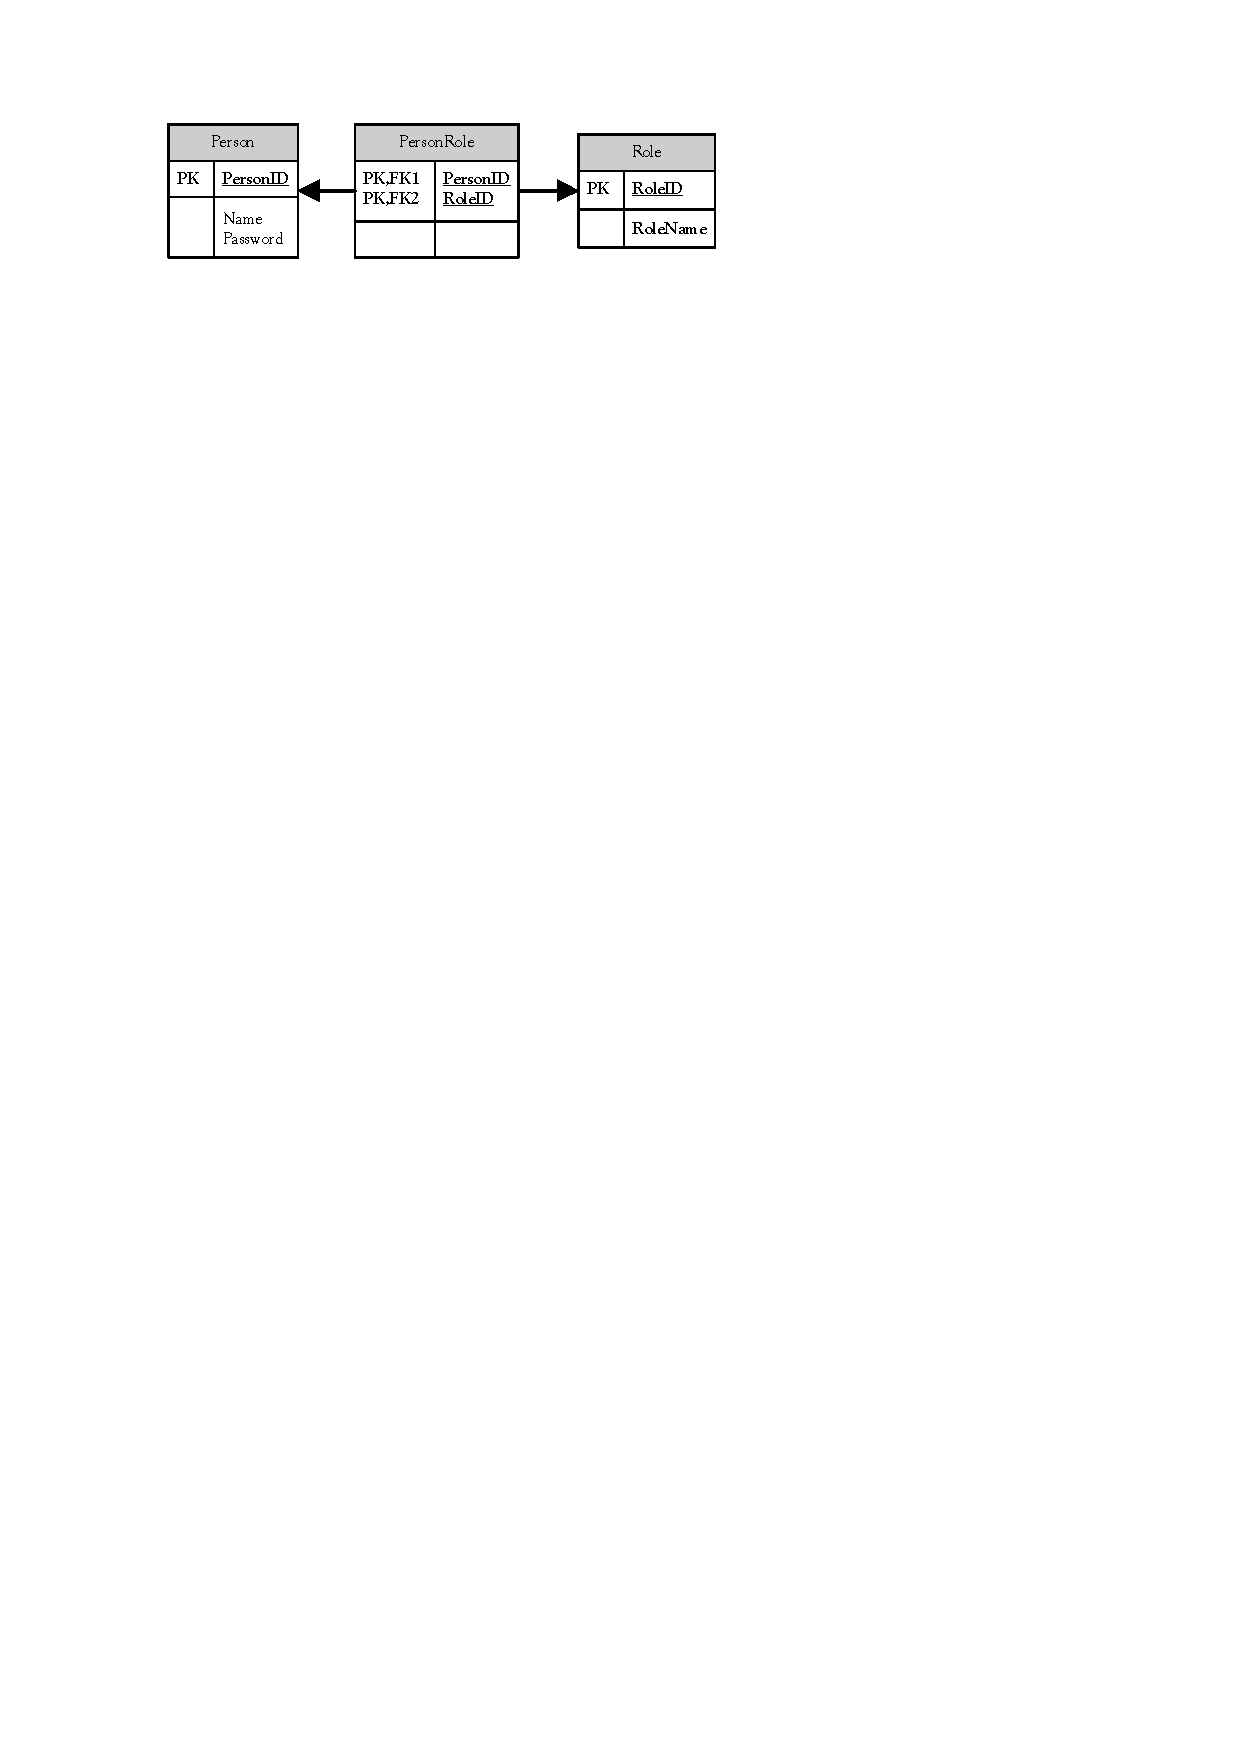
\includegraphics{./files/inc/figures/AnalysisEnumNew}
				\caption{\label{fig:AnalysisEnumNew} normalized database}
			\end{center}
		\end{figure}
	
	
	%-----
	\section{Lookup tables}

		An enum is not dedicated to present a description to the user. Every text 
		representing a database entry has to come out of the database. So you can 
		avoid consistency problem between code and database.
		
		Descriptions for numeric ids are always references to so called lookup 
		table. You can add all descriptions to one table or use one tables for each 
		relation. With a little effort it is even possible to save the values in 
		different languages.
				
		To change, add and remove the values you don't have to recompile the code 
		but only change the entries in the database. Another advantage of a lookup 
		table is the flexibility of such a table. 
		
		In Figure \ref{fig:AnalysisEnumExtended} you can see two tables which has 
		its descriptions in the same table. The table Car has the names of colors 
		and the table PersonRole its role names in the EnumLookup table. This 
		descriptions can be added for different languages. The names of languages 
		are defined in the Language table.
		
		\begin{figure}[hbt]
			\begin{center}
				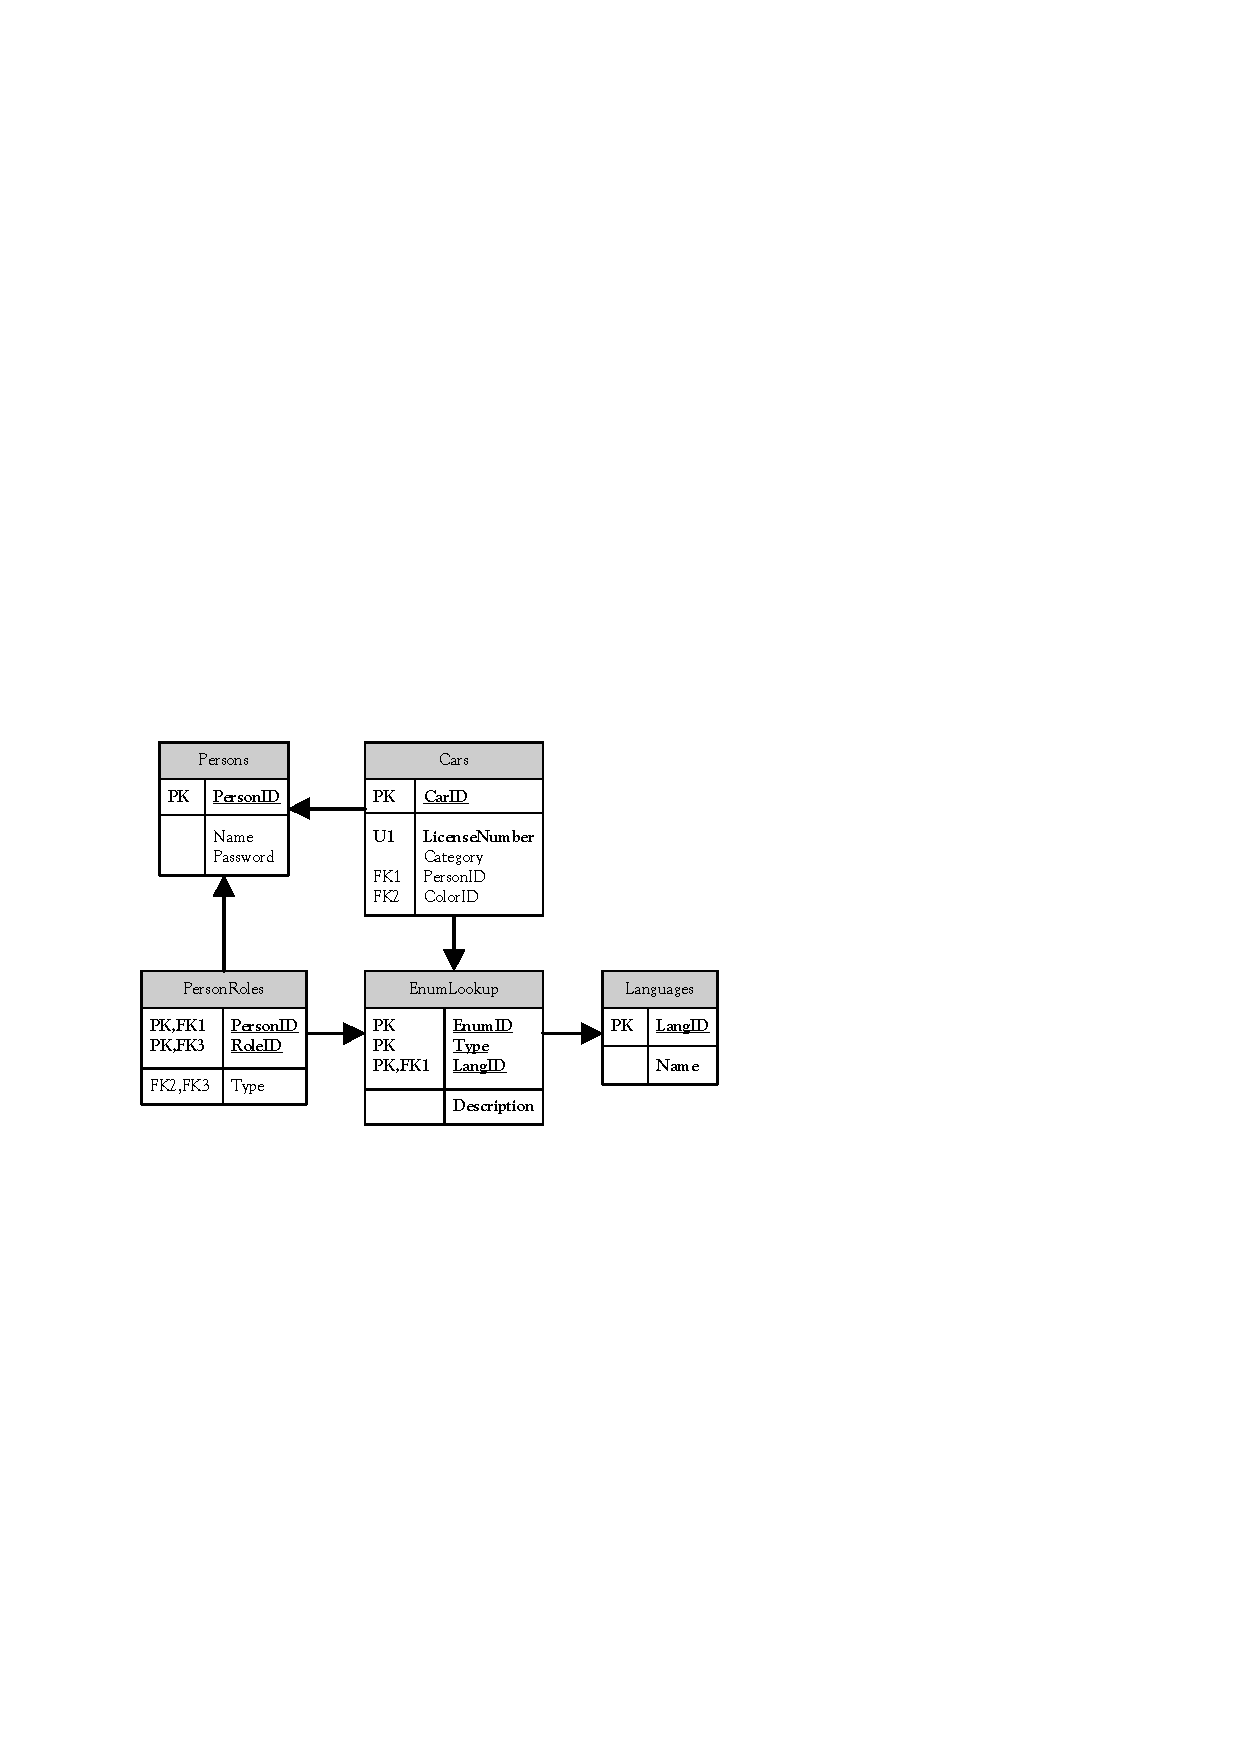
\includegraphics{./files/inc/figures/AnalysisEnumExtended}
				\caption{\label{fig:AnalysisEnumExtended} lookup table}
			\end{center}
		\end{figure}
		
		If descriptions of different tables are saved in one lookup table, you will 
		need to know which descriptions belong to which table. There are two 
		possibilities. You could define ranges of the ID belonging to a table. But 
		the better solution is to add a description type to the lookup table as you 
		can see in Figure \ref{fig:AnalysisEnumExtended}. That is one of the rare cases 
		where you could use an enum in the database if provided, because this values 
		will only be used in the code. The user will never see it.
		
		%-----
		\section{Loading lookup table data}
		
		There are several strategies to load data from lookup tables. Due to the fact this 
		data often are nearly static, it could be a good deal to read the data once 
		and hold in memory. 
		
		Another possibility is to get the values within one request. In Listing \ref{lst:enumJoinTables}
		you see an example of joining the tables. This statement can be used directly or by 
		creating a view on the database.
		
		\begin{lstlisting}[float=hbt,language={SQL},caption=join tables,label=lst:enumJoinTables]
SELECT c.LicenseNumber, p.Name, e.Description AS Color
FROM Cars AS c
	LEFT OUTER JOIN Persons AS p
		ON c.PersonID = p.PersonID
	LEFT OUTER JOIN EnumLookup AS e
		ON c.ColorID = e.EnumID
			AND EnumLookup.Type = 'cars'
			AND EnumLookup.LangID = 1
WHERE c.Category = 1
		\end{lstlisting}